\chapter{プログラム解説}
本章では,今回作成したプログラムをライブラリ化し継続的な発展が可能なようにそれぞれの処理の解説を記述する.

\section{アルゴリズム}
分子動力学法を用いて粒子を動かしていくアルゴリズムは以下のようになる.
\begin{enumerate}
  \item 複数の粒子モデルを用意し,現在の座標、1つ前の座標,粒子に加わる力のパラメータを持たせる.
  \item Lennard-Jonesポテンシャルを用いて,粒子モデルに加わる力の合力を計算する.
  \item Verlet法を用いて次の座標を計算する.
  \item 2-3を繰り返して粒子モデルの座標を継続的に決定し続ける.
\end{enumerate}


\section{粒子の初期状態の設定}
粒子の座標,粒子にかかっている力を初期状態にする関数set\_particleは以下のように実装した.
\begin{screen}
{\small
\begin{verbatim}
void set_particle(){
  int i, j, k=0;
  for(i=1; i<10; i++){
    for(j=1; j<10; j++){
      if(k==n) break;
      ball_p[k][0] = i;
      ball_p[k][1] = j;
      pre_p[k][0] = i;
      pre_p[k][1] = j;
      k++;
    }
  }
  for(i=0; i<n; i++){
    ball_f[i][0] = 0; 
    ball_f[i][1] = 0;
  } 
} 
\end{verbatim}}
\end{screen}
変数i, jは粒子の座標を等間隔にするための任意の数値であり,kは粒子の番号,nは粒子の個数である.
粒子の数だけ,粒子の座標(ball\_p)と過去の座標(pre\_p)の初期値の格納を行い,粒子にかかっている力(ball\_f)を初期状態の0に設定している.
座標の初期値は左上から縦に9個ずつ等間隔に並ぶようになる.この関数はリセットにも用いられており,スライダーによって粒子の数が変更された際も実行される.

\section{粒子に加わる力}
ある一つの粒子に加わる力を決定するためには,他の粒子それぞれに対して力の計算を行い,それらの合力を求める必要がある.
\subsection{粒子間に加わる力の計算}
粒子間距離からLennard-Jonesポテンシャルを用いて,粒子に加わる力を求める.2粒子の座標からそれぞれの粒子に加わる力を計算する関数inter\_forceは以下ように実装した.
\begin{screen}
{\small
\begin{verbatim}
float[] lennard(float p1[], float p2[]){
  float d, force;
  float[] force_xy = new float[2];
  d = distance(p1, p2);
  force = -30 * pow(d,-13) + 30 * pow(d,-7);
  force_xy[0] = force * (p2[0] - p1[0])/d; 
  force_xy[1] = force * (p2[1] - p1[1])/d;
  return force_xy;  
}
\end{verbatim}}
\end{screen}
粒子の座標p1,p2を引数とし,p1に加わる力を返すようになっている.force\_xy[0]はx方向成分, force\_xy[1]はy方向成分である.
Lennard-Jonesポテンシャルによる力の計算は粒子間距離が1の時に力が0になるように定数を決めている.
粒子p2に加わる力はp1に加わる力の逆向きになるので以下のような実装を行う.
\begin{screen}
{\small
\begin{verbatim}
void inter_force(int i, int j){
  float[] tmp= new float[2];
  tmp = lennard(ball_p[i], ball_p[j]);
  ball_f[i][0] += tmp[0];
  ball_f[i][1] += tmp[1];
  ball_f[j][0] += -tmp[0];
  ball_f[j][1] += -tmp[1];
}
\end{verbatim}}
\end{screen}
2つの粒子の番号を引数とし,それらの粒子の座標を用いて関数lennardを実行し,結果をそれぞれのball\_fに格納している.後に複数の粒子との合力を求めるためにball\_fに対して加算代入(+=)を行う.
\subsection{合力の計算}
\begin{screen}
{\small
\begin{verbatim}
for( i=0; i<n-1; i++){
  for( j=i+1; j<n; j++){
    inter_force(i, j);
  }
}
\end{verbatim}}
\end{screen}
n個の粒子に対して重複を持たないように2粒子組み合わせを全て選択し,関数inter\_forceを実行している.これによりそれぞれの粒子のball\_fに,粒子間に加わる力が何度も加算代入され合力が求まる.

\section{粒子の動作}
粒子の座標の計算を行い,座標を更新することによって粒子を動かしていく.
\subsection{Verlet法による計算}
Verlet法を用いて粒子の座標を決定する.Verlet法の計算は以下のように実装した.
\begin{screen}
{\small
\begin{verbatim}
float[] verlet(float current[], float previous[], float force[]){
  float[] newpos = new float[2];
  newpos[0]=2*current[0]-previous[0]+h*h/m*force[0];
  newpos[1]=2*current[1]-previous[1]+h*h/m*force[1];
  return newpos;
} 
\end{verbatim}}
\end{screen}
Verlet法に従い,現在の座標(current),h時間前の座標(previous),粒子にかかっている力(force)を引数として,h時間後の座標(newpos)を返すようになっている.hは時間刻み,mは質量であり,それぞれグローバル変数で定義している.
\subsection{座標の更新}
Verlet法の計算結果から粒子の座標を更新する関数は以下のように実装した.
\begin{screen}
{\small
\begin{verbatim}
void calc_verlet(int i){
  float[] tmp= new float[2];
  if(solid_mode) ball_f[i][1]+= 0.00001/(h*h);//solid_mode
  tmp = ball_p[i];
  ball_p[i] = verlet(ball_p[i], pre_p[i],ball_f[i]);
  pre_p[i]= tmp; 
}
\end{verbatim}}
\end{screen}
i番目の粒子に対してVerlet法の計算を行い,計算結果から現在の座標(ball\_p)の更新を行う.Verlet法を繰り返し行えるように過去の座標(pre\_p)の更新も行う必要があり,tmpを用いて更新前のball\_pをpre\_pに格納している.

\section{粒子の描画}
粒子の座標が決定したので,粒子の描画を行う.また,粒子の速度によって色を変化させる.
\begin{screen}
{\small
\begin{verbatim}
void draw_particle(int i){
  float v;
  v = distance(ball_p[i], pre_p[i]);
  colorMode(HSB,360,100,100);
  fill(230+5000*v,100,100);  
  ellipse(ball_p[i][0]*50,ball_p[i][1]*50, ball_size*100,ball_size*100);
}
\end{verbatim}}
\end{screen}

\subsection{描画}
\begin{screen}
{\small
\begin{verbatim}
ellipse(ball_p[i][0]*50,ball_p[i][1]*50, ball_size*100,ball_size*100);
\end{verbatim}}
\end{screen}
粒子の描画はball\_p*50ピクセルの位置に円を描くというものになる.50倍するのはball\_pの値の範囲が0から10であり,粒子の動作範囲が500ピクセルの正方形であるからである.ball\_sizeは粒子のサイズを決定するグローバル変数である.

\subsection{粒子の色}
粒子の速度によって色を変化させる.色は速度が大きくなればなるほど,青から赤に変化するようにする.
\begin{screen}
{\small
\begin{verbatim}
  float v;
  v = distance(ball_p[i], pre_p[i]);
  colorMode(HSB,360,100,100);
  fill(230+5000*v,100,100); 
\end{verbatim}}
\end{screen}
粒子の現在の座標(ball\_p)と過去の座標(pre\_p)の距離を速度と考え,それに応じて色を変化させるようにしている.カラーモードをHSBに変更することによって,H(色相)の調整のみで青から赤に変化させる事が可能になる.

\begin{figure}[htbp]
 \begin{center}
  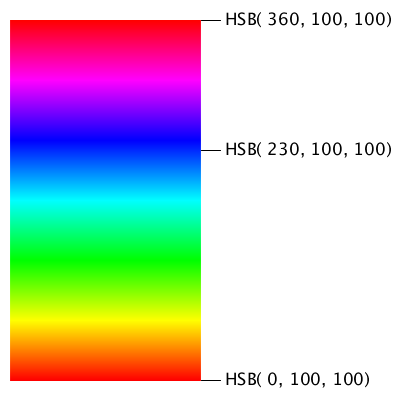
\includegraphics[width=80mm]{../implement/color_HSB.png}
 \end{center}
 \caption{HSBによる色の変化.}
 \label{fig:hsb}
\end{figure}
図\ref{fig:hsb}はS(彩度)=100,B(明度)=100の状態でH(色相)を変化させたときの色の変化を表している.粒子の色は230から360までの値をとり,青から赤に徐々に変化することが確認できる.

\section{壁との衝突}
粒子が動作範囲内の枠内を超えた場合,衝突判定を行い反射させる必要がある.判定を行う関数reflectは以下のように実装した.
\begin{screen}
{\small
\begin{verbatim}
void reflect(int i){
  if(ball_p[i][0]<ball_size){
  ball_p[i][0] = ball_size*2-ball_p[i][0];
  pre_p[i][0] = ball_size*2-pre_p[i][0];
  }  
  else if(ball_p[i][0]>10-ball_size){
    ball_p[i][0] = (10-ball_size)*2-ball_p[i][0];
    pre_p[i][0] = (10-ball_size)*2-pre_p[i][0];
  }

  if(ball_p[i][1]<ball_size){
    ball_p[i][1] = ball_size*2-ball_p[i][1];
    pre_p[i][1] = ball_size*2-pre_p[i][1];
  }
  else if(ball_p[i][1]>10-ball_size && solid_mode)
   ball_p[i][1]=10-ball_size-0.01;  
  else if(ball_p[i][1]>10-ball_size){
    ball_p[i][1] = (10-ball_size)*2-ball_p[i][1];
    pre_p[i][1] = (10-ball_size)*2-pre_p[i][1];
  }
}
\end{verbatim}}
\end{screen}
粒子iについて壁との衝突判定を行い,反射させている.衝突判定は上下左右の壁と行う必要があり,if文でそれぞれ行っている.
粒子の動きはVerlet法で定めているので,現在の座標(ball\_p)だけを更新しても,それ以降のVerlet法の計算に支障がでてしまう.そのため反射角が合うように過去の座標(pre\_p)の更新も行う.

\begin{figure}[htbp]
 \begin{center}
  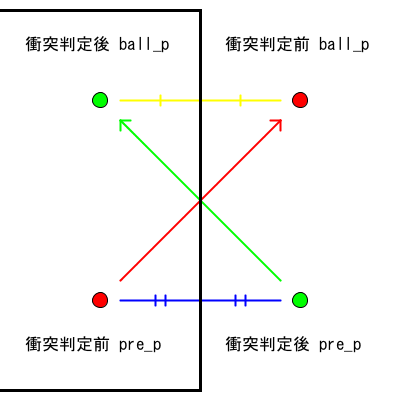
\includegraphics[width=80mm]{../implement/reflect_picture.png}
 \end{center}
 \caption{衝突判定時の座標の変換.}
 \label{fig:reflect}
\end{figure}

図\ref{fig:reflect}は衝突前後の粒子の座標を表しており,赤い粒子が衝突判定前,緑の粒子が衝突判定後を示しており,黄と青の線はそれぞれの粒子が壁と同じ距離であることを示している.
このような座標の変換をすることによって自然な衝突を表現できる.

\clearpage
\section{選択した粒子に力を加える}
クリックされた粒子にドラッグした方向の力を加えるようにし,ドラッグの距離によって力の大きさを変えるようにする.以下のように実装した.
\begin{screen}
{\small
\begin{verbatim}
int click_ball=0;

void mousePressed() {
  int i;
  for(i=0; i<n; i++){
    if(mouseX-10-20<=ball_p[i][0]*50 & mouseX-10+20>= ball_p[i][0]*50 &
    mouseY-10-20<=ball_p[i][1]*50 & mouseY-10+20>= ball_p[i][1]*50){
      click_ball = i;
      fill(0);
      //Ver Processing
      ellipse(pre_p[i][0]*50,pre_p[i][1]*50,ball_size*100,ball_size*100); 
      /*Ver JavaScript
      ellipse(10+pre_p[i][0]*50,10+pre_p[i][1]*50, 
       ball_size*100,ball_size*100);
       */
      mouse_p[0] = mouseX;
      mouse_p[1] = mouseY;
      return;
    }
  }
  click_ball = -1;
}
void mouseReleased(){
  if(click_ball != -1){
    ball_f[click_ball][0] +=( mouseX - mouse_p[0])*0.0001/(h*h);
    ball_f[click_ball][1] += (mouseY - mouse_p[1])*0.0001/(h*h);
  }
}
\end{verbatim}}
\end{screen}

\subsection{粒子の選択}
粒子がクリックされているかの判定を行い,クリックされていた場合,何番目の粒子か確認する必要がある.
また,選択された粒子がわかりやすいように黒く描画する.
\begin{screen}
{\small
\begin{verbatim}
void mousePressed() {
  int i;
  for(i=0; i<n; i++){
    if(mouseX-10-20<=ball_p[i][0]*50 & mouseX-10+20>= ball_p[i][0]*50 &
    mouseY-10-20<=ball_p[i][1]*50 & mouseY-10+20>= ball_p[i][1]*50){
      click_ball = i;
      fill(0);
      //Ver Processing
      ellipse(pre_p[i][0]*50,pre_p[i][1]*50,ball_size*100,ball_size*100); 
      /*Ver JavaScript
      ellipse(10+pre_p[i][0]*50,10+pre_p[i][1]*50, 
       ball_size*100,ball_size*100);
       */
      mouse_p[0] = mouseX;
      mouse_p[1] = mouseY;
      return;
    }
  }
  click_ball = -1;
}
\end{verbatim}}
\end{screen}
マウスボタンが押下された際に,i番目の粒子の上にマウスポインタが重なっているかの判定を行う.これをn個の粒子全てに対して行っていき
\begin{itemize}
  \item 重なりを確認した場合
\end{itemize}

\begin{enumerate}
 \setlength{\leftskip}{1.0cm}
  \item click\_ballに粒子の番号を格納する.
  \item その粒子を黒く描画する.
  \item マウスポインタの座標をmouse\_pに格納する.
  \item 関数mouse\_Pressedを終了する.
\end{enumerate}

\begin{itemize}
  \item 粒子全てに対して重なりを確認できなかった場合
\end{itemize}

\begin{itemize}
   \setlength{\leftskip}{1.0cm}
  \item click\_ballに-1を格納する.
\end{itemize}
この処理によりclick\_ballには選択された粒子の番号か-1が格納されている.また粒子が選択された場合,mouse\_pにはマウスポインタの座標が格納されている.これらの値はマウスが離された際の処理で利用する事になる.またProcessingとJavaScriptでの動作に異なりが生じるため変換を行う際は,プログラム内のコメントアウト部分の書き換えを行う必要がある.

\subsection{ドラッグ後の処理}
\begin{screen}
{\small
\begin{verbatim}
void mouseReleased(){
  if(click_ball != -1){
    ball_f[click_ball][0] +=( mouseX - mouse_p[0])*0.0001/(h*h);
    ball_f[click_ball][1] += (mouseY - mouse_p[1])*0.0001/(h*h);
  }
}
\end{verbatim}}
\end{screen}
マウスボタンが押された際に格納しておいたclick\_ball,mouse\_pを利用する.
マウスボタンが離された際にclick\_ballが-1以外(粒子が選択されている状態)であれば,ドラッグされた距離に応じてball\_f[click\_ball]に力を加える.このような実装を行う事でマウスボタンを用いて粒子を扱うことが可能になる.
また,格納する力の値を$h^2$で割っているのは時間刻みhの大きさに合わせて力の大きさを調整する必要があるからである.

\section{キー入力}
\begin{screen}
{\small
\begin{verbatim}
boolean solid_mode = false;
boolean force_mode = false;

void keyPressed() {  
  if (key == 's'||key == 'S') {
    if(solid_mode) solid_mode = false;
    else solid_mode = true;
  }
      if (key == 'f'||key == 'F') {
    if(force_mode) force_mode = false;
    else force_mode = true;
  }
  if (key == 'r'||key == 'R') set_particle();
}
\end{verbatim}}
\end{screen}
boolean変数がキー入力に対してtrue,falseと切り替わり,モード変更が可能になる.今回はSキーで凝固状態(solid\_mode),Fキーで力を視覚化した状態(force\_mode)の切り替えを行う.
またRキーはリセットに対応していて,粒子の状態を初期化する関数set\_particleを実行する.

\section{凝固状態}
凝固の現象を擬似的に表すために粒子に常に下向きの力を加え下層部に溜まるようにする.また,枠の下面部に粒子が衝突した際の反発力を減らす処理を行う.
\begin{itembox}[c]{関数calc\_verlet内 下向きの力を加える処理}
{\small
\begin{verbatim}
if(solid_mode) ball_f[i][1]+= 0.00001/(h*h);
\end{verbatim}}
\end{itembox}

\begin{itembox}[c]{関数reflect内 下面部の枠の反発力を減らす処理}
{\small
\begin{verbatim}
else if(ball_p[i][1]>10-ball_size && solid_mode)
 ball_p[i][1]=10-ball_size-0.01;
\end{verbatim}}
\end{itembox}
これらの処理はsolid\_modeがtrueの場合実行される.下面部の反発力を減らす処理では,粒子が下面部を通り越した際に,粒子のy座標に下面部と接触するようなy座標を格納している.これにより衝突後の反発力を減らすことができる.
この処理は粒子が壁と接触するように座標を決定するため反発力を0にしているように思えるが,継続的に下向きの力が加えられた状態でverlet法での計算が行われるため粒子に多少の上向きの動きが生じるようになる.
また,これを以下のように書き換えると反発力を0にすることができる.
\begin{screen}
{\small
\begin{verbatim}
else if(ball_p[i][1]>10-ball_size && solid_mode) {
  ball_p[i][1]=10-ball_size-0.01; 
  pre_p[i][1]=10-ball_size-0.01;   
}
\end{verbatim}}
\end{screen}
反発力を0にしてしまうと粒子が最下層に詰まってしまい粒子間距離が近すぎてしまう.この振る舞いは凝固の表現には不適切である.そのため,反発力を0にせずに少し減らす処理を選択した.

\section{力を視覚化した状態}
粒子に加わる力を線を用いて表す関数draw\_forceは以下のように実装した.
\begin{screen}
{\small
\begin{verbatim}
void draw_force(int i){
  float force_sqrt_x, force_sqrt_y;
  strokeWeight(3);
  if(ball_f[i][0]>0) force_sqrt_x = sqrt(abs(ball_f[i][0]));
  else force_sqrt_x = -sqrt(abs(ball_f[i][0]));
  if(ball_f[i][1]>0) force_sqrt_y = sqrt(abs(ball_f[i][1]));
  else force_sqrt_y = -sqrt(abs(ball_f[i][1]));
  line(ball_p[i][0]*50, ball_p[i][1]*50,
   ball_p[i][0]*50+force_sqrt_x, ball_p[i][1]*50+force_sqrt_y);
  strokeWeight(1);
}
\end{verbatim}}
\end{screen}
粒子iの座標(ball\_p[i][0]*50, ball\_p[i][1]*50)を始点とし,始点+粒子に加わっている力の根号(ball\_p[i][0]*50+force\_sqrt\_x ,ball\_p[i][1]*50+force\_sqrt\_y)まで太めの線(strokeWeight(3))の描画を行う.
粒子に加わっている力は振れ幅が大きいため根号を用いている.これにより1以下の小さな値の変化が確認しやすくなる.
粒子に加わる力には負の値も存在するが,根号の計算では負の値を扱うことができない.そのため,粒子に加わる力の絶対値から根号を求め,その値の符号を元の値と同一にする必要がある.
sqrt(abs(ball\_f[i][0]))はx方向に加わる力の絶対値の根号であり,粒子に加わる力の符号と同じになるようにforce\_sqrt\_xに格納している.
今回は線の長さに根号を用いているが,値をそのまま利用する方法もある.この方法には力の大きさが長さに比例するという利点があり,以下のように書き換えればよい.
\begin{screen}
{\small
\begin{verbatim}
line(ball_p[i][0]*50,ball_p[i][1]*50,
 ball_p[i][0]*50+ball_f[i][0],ball_p[i][1]*50+ball_f[i][1]);
\end{verbatim}}
\end{screen}



\section{スライダー}\label{sec:slider}
\begin{screen}
{\small
\begin{verbatim}
float slider_value = 1;
boolean slider_dragged = false;

void slider(int position_x, int position_y, int slider_height,
  int slider_width, int min, int max, int NumberOfTickMarks){
  
  int num_separator =
    (int)map(slider_value, min, max, 0, NumberOfTickMarks-1);
  float cordinate_y = position_y + slider_height - 
    ((float)slider_height / (NumberOfTickMarks-1))*num_separator;
  fill(255);
  rect(position_x, position_y, slider_width, slider_height);
  fill(0);
  rect(position_x, cordinate_y, slider_width, position_y +
    slider_height - cordinate_y);
  
  text( slider_value, position_x, position_y + slider_height + 20);
  
  
  if(mouseX >= position_x & mouseX <= position_x + slider_width &
    mouseY<=cordinate_y+10 & mouseY>= cordinate_y-10){
    if (mousePressed){
      slider_dragged= true;
    }
   }
  if(mousePressed==false) slider_dragged=false; 
   
   if(slider_dragged){
     num_separator+= (int)((cordinate_y - mouseY)/
       ((float)slider_height / (NumberOfTickMarks-1)));
     num_separator = constrain(num_separator, 0, NumberOfTickMarks-1);
     slider_value=map(num_separator, 0, NumberOfTickMarks-1, min, max);
   }
}
\end{verbatim}}
\end{screen}

\newpage

このプログラムを利用するためにはスライダーの値を格納する変数slider\_valueとスライダーのクリック判定を行う変数slider\_draggedをグローバル変数で定義する必要がある.
関数sliderの引数はスライダーの左上の座標を決定するposition\_x,position\_y,縦と横の幅を決定するslider\_height, slider\_width, 
値の最小値,最大値を決定するmin, max, 区切りの数を決定するNumberOfTickMarksとなり,それらを宣言することでスライダーを利用できる.
変数num\_separatorにはスライダーの一番下を0番目として区切りが下から何番目なのかを格納している.
この整数の値を利用することによってマウスをドラッグした際のスライダーの区切りを表現することができる.
以下にプログラムの処理の流れを記す.

\begin{enumerate}
  \item スライダーの値(slider\_value)から,区切りが下から何番目か(num\_separator)を計算する.
  \item 区切りの番号から,スライダー部分のy座標(cordinate\_y)を計算する.
  \item スライダーを描画する.
  \item スライダーの掴み判定(slider\_dragged)を行う.
   \item 掴み判定がtrueの場合
\end{enumerate}

\begin{enumerate}
   \setlength{\leftskip}{1.0cm}
  \item マウスの移動距離に合わせて区切りの番号に値を加える.
  \item 区切りの番号からスライダーの値を計算し格納する.
\end{enumerate}


\if0

\subsection{粒子の初期状態の設定}
\subsubsection{粒子の初期状態の設定}
\begin{screen}
{\small
\begin{verbatim}

\end{verbatim}}
\end{screen}
\fi

%\end{document}

